% Requires llncs.cls from Springer LNCS template
% Download from: https://www.springer.com/gp/computer-science/lncs/conference-proceedings-guidelines
\documentclass[runningheads]{llncs}

\usepackage{graphicx}
\usepackage{amsmath}
\usepackage{amssymb}
\usepackage{booktabs}
\usepackage[ruled,vlined]{algorithm2e}
\usepackage{hyperref}
\usepackage{xcolor}
\usepackage{multirow}
\usepackage{tikz}
\usetikzlibrary{shapes.geometric, arrows.meta, positioning, fit, backgrounds}

\begin{document}

\title{AARS: Agentic Adaptive Retrieval for Dynamic Strategy Selection in Retrieval-Augmented Generation}

\author{Anonymous Authors}
\institute{Anonymous Institution}

\maketitle

%% ============================================================
%% ABSTRACT
%% ============================================================
\begin{abstract}
Retrieval-Augmented Generation (RAG) systems typically employ a fixed retrieval strategy regardless of query characteristics, leading to suboptimal performance across diverse question types. Factual queries benefit from keyword precision, analytical queries require semantic depth, and multi-hop queries demand iterative graph traversal---yet no single retriever handles all cases well. We present AARS (Agentic Adaptive Retrieval System), a framework that uses LLM-based planner and reflection agents to dynamically select retrieval strategies on a per-query basis. AARS introduces four key contributions: (1)~an agentic planner that classifies queries and selects from keyword, vector, graph, or hybrid retrieval strategies; (2)~a reflection agent that iteratively evaluates retrieval sufficiency and triggers re-retrieval with modified strategies when needed; (3)~a fusion pipeline combining Reciprocal Rank Fusion with Maximal Marginal Relevance for cross-strategy result merging; and (4)~comprehensive evaluation across four standard benchmarks. Experiments on HotpotQA, Natural Questions, TriviaQA, and MS~MARCO demonstrate that AARS achieves 3--8\% improvement in Token~F1 over static retrieval baselines and 2--5\% improvement over existing adaptive retrieval methods, with the largest gains observed on multi-hop reasoning tasks. Our analysis reveals that the planner agent correctly adapts strategy selection to query complexity, while the reflection mechanism recovers from initial retrieval failures in 34\% of insufficient-retrieval cases.

\keywords{Retrieval-Augmented Generation \and Adaptive Retrieval \and Multi-Strategy Retrieval \and LLM Agents \and Question Answering}
\end{abstract}

%% ============================================================
%% 1. INTRODUCTION
%% ============================================================
\section{Introduction}
\label{sec:introduction}

Retrieval-Augmented Generation (RAG)~\cite{Lewis2020} has emerged as a dominant paradigm for grounding large language model (LLM) outputs in external knowledge. By retrieving relevant documents at inference time and conditioning generation on retrieved passages, RAG systems reduce hallucination and enable access to up-to-date information without costly model retraining~\cite{Guu2020,Borgeaud2022}. However, the vast majority of deployed RAG systems rely on a single, static retrieval strategy---typically dense passage retrieval---applied uniformly to all incoming queries.

This one-size-fits-all approach is fundamentally mismatched with the diversity of real-world information needs. Consider three representative query types: (1)~\textit{``Who invented the transistor?''}---a factual query where keyword matching on ``transistor'' and ``invented'' would yield precise results; (2)~\textit{``How do attention mechanisms relate to memory in neural networks?''}---an analytical query requiring semantic understanding of conceptual relationships; and (3)~\textit{``What awards has the director of Inception received for films produced by Legendary Pictures?''}---a multi-hop query requiring entity resolution and relationship traversal across multiple documents. No single retrieval strategy optimally serves all three.

Recent work has begun addressing this limitation through adaptive retrieval approaches. FLARE~\cite{Jiang2023} triggers retrieval based on generation confidence, Self-RAG~\cite{Asai2023} learns reflection tokens to assess retrieval quality, and Adaptive-RAG~\cite{Jeong2024} uses a classifier to route queries by complexity. However, these approaches either (a)~adapt only the \textit{timing} of retrieval rather than the \textit{strategy}, (b)~require specialized training, or (c)~use simple heuristic routing without the reasoning capabilities of modern LLMs.

In this paper, we introduce AARS (\textbf{A}gentic \textbf{A}daptive \textbf{R}etrieval \textbf{S}ystem), a framework that \textit{thinks before retrieving} by employing LLM-based agents for dynamic strategy selection. Our key insight is that the same language understanding capabilities that power modern LLMs can be leveraged to analyze query characteristics and select appropriate retrieval strategies---a task that requires the kind of nuanced reasoning that rule-based approaches struggle with.

Our contributions are fourfold:

\begin{enumerate}
    \item \textbf{Agentic Planning}: We introduce a planner agent that uses structured LLM output to classify queries along multiple dimensions (type, complexity) and select from keyword, vector, graph, hybrid, or no-retrieval strategies, with optional query decomposition for multi-hop reasoning.

    \item \textbf{Reflective Re-retrieval}: We propose a reflection agent that evaluates whether retrieved documents are sufficient to answer the query, triggering iterative re-retrieval with modified queries and strategies when initial retrieval is inadequate.

    \item \textbf{Cross-Strategy Fusion}: We design a two-stage fusion pipeline combining Reciprocal Rank Fusion (RRF)~\cite{Cormack2009} for cross-retriever score normalization with Maximal Marginal Relevance (MMR)~\cite{Carbonell1998} for diversity-aware reranking.

    \item \textbf{Comprehensive Evaluation}: We evaluate AARS on four standard benchmarks (HotpotQA, Natural Questions, TriviaQA, MS~MARCO) against five baselines and conduct ablation studies demonstrating the contribution of each component.
\end{enumerate}

The remainder of this paper is organized as follows. Section~\ref{sec:related_work} reviews related work on RAG and adaptive retrieval. Section~\ref{sec:methodology} presents the AARS architecture in detail. Sections~\ref{sec:experiments} and~\ref{sec:results} describe our experimental setup and results. Section~\ref{sec:discussion} discusses findings and limitations. Section~\ref{sec:conclusion} concludes with future directions.

%% ============================================================
%% 2. RELATED WORK
%% ============================================================
\section{Related Work}
\label{sec:related_work}

\subsection{Retrieval-Augmented Generation}

The foundational RAG framework by Lewis et al.~\cite{Lewis2020} combines a pre-trained Dense Passage Retriever (DPR)~\cite{Karpukhin2020} with a BART generator, training the retriever end-to-end for downstream tasks. Subsequent work has extended this paradigm along several dimensions: REALM~\cite{Guu2020} pre-trains with a retrieval component, RETRO~\cite{Borgeaud2022} scales retrieval to trillions of tokens, FiD~\cite{Izacard2021} processes multiple passages through fusion-in-decoder, and REPLUG~\cite{Shi2023} treats the LLM as a black box with retrieval prepended to the input. These approaches share a common limitation: they employ a single, fixed retrieval mechanism regardless of query characteristics.

\subsection{Active and Adaptive Retrieval}

A growing body of work addresses \textit{when} and \textit{how} to retrieve. FLARE~\cite{Jiang2023} implements forward-looking active retrieval, monitoring generation confidence token-by-token and triggering retrieval when uncertainty exceeds a threshold. While effective for long-form generation, FLARE adapts retrieval \textit{timing} but not \textit{strategy}---it always uses the same retriever.

Self-RAG~\cite{Asai2023} takes a different approach by training the language model to generate special reflection tokens (\texttt{[Retrieve]}, \texttt{[IsRel]}, \texttt{[IsSup]}, \texttt{[IsUse]}) that control retrieval decisions and assess passage relevance. This enables the model to self-assess retrieval quality, but requires specialized training with reflection token annotations.

Adaptive-RAG~\cite{Jeong2024} most closely resembles our approach, using a trained classifier to route queries into simple (no retrieval), moderate (single-step), or complex (multi-step) categories. However, it uses a small trained classifier rather than leveraging the reasoning capabilities of LLMs for strategy selection, and it does not consider multiple retrieval modalities (keyword, vector, graph).

CRAG (Corrective RAG)~\cite{Yan2024} introduces a lightweight retrieval evaluator that assesses document relevance and triggers web search as a corrective mechanism when initial retrieval fails. While CRAG shares our motivation for retrieval quality assessment, it is limited to a binary correct/incorrect evaluation and a single corrective action.

Our approach differs from all of the above by combining three capabilities: (1)~LLM-based reasoning for strategy selection across multiple retrieval modalities, (2)~iterative reflection with strategy adaptation, and (3)~multi-strategy fusion. Table~\ref{tab:related_comparison} summarizes these distinctions.

\begin{table}[t]
\centering
\caption{Comparison of AARS with related adaptive retrieval approaches.}
\label{tab:related_comparison}
\begin{tabular}{lccccc}
\toprule
\textbf{System} & \textbf{Multi-Strategy} & \textbf{LLM Planning} & \textbf{Reflection} & \textbf{Fusion} & \textbf{Training-Free} \\
\midrule
FLARE~\cite{Jiang2023} & \texttimes & \texttimes & \texttimes & \texttimes & \checkmark \\
Self-RAG~\cite{Asai2023} & \texttimes & \texttimes & \checkmark & \texttimes & \texttimes \\
Adaptive-RAG~\cite{Jeong2024} & \texttimes & \texttimes & \texttimes & \texttimes & \texttimes \\
CRAG~\cite{Yan2024} & \texttimes & \texttimes & \checkmark & \texttimes & \checkmark \\
\textbf{AARS (ours)} & \checkmark & \checkmark & \checkmark & \checkmark & \checkmark \\
\bottomrule
\end{tabular}
\end{table}

\subsection{Multi-Strategy Retrieval and Fusion}

Hybrid retrieval combining sparse (BM25~\cite{Robertson2009}) and dense (embedding-based~\cite{Reimers2019}) retrievers has shown consistent improvements over either approach alone. Reciprocal Rank Fusion (RRF)~\cite{Cormack2009} provides a simple yet effective method for combining ranked lists from heterogeneous sources using the formula $\text{score}(d) = \sum_r \frac{1}{k + \text{rank}_r(d)}$, where $k$ is a smoothing constant. Maximal Marginal Relevance (MMR)~\cite{Carbonell1998} addresses result diversity by iteratively selecting documents that balance relevance with novelty relative to already-selected documents.

While hybrid search is well-established, existing systems typically use a fixed combination of exactly two retrievers (sparse + dense) with static fusion weights. AARS extends this paradigm to four retrieval modalities and dynamically selects which combination to employ based on query analysis.

%% ============================================================
%% 3. METHODOLOGY
%% ============================================================
\section{Methodology}
\label{sec:methodology}

\subsection{System Overview}

AARS processes queries through a multi-stage pipeline orchestrated by two LLM-based agents. Figure~\ref{fig:architecture} illustrates the architecture. Given a user query $q$, the system executes the following stages:

\begin{enumerate}
    \item The \textit{Planner Agent} analyzes $q$ and produces a retrieval plan specifying the strategy, an optimized query, and optional sub-queries for decomposition.
    \item The \textit{Retrieval Layer} executes the selected strategy using the appropriate retriever(s).
    \item The \textit{Reflection Agent} evaluates whether the retrieved documents $D$ are sufficient; if not, it modifies the query and strategy for re-retrieval (up to $T$ iterations).
    \item The \textit{Fusion Pipeline} merges and reranks results across retrieval iterations and strategies.
    \item The \textit{Answer Generator} produces a grounded response with citations.
\end{enumerate}

\begin{figure}[t]
\centering
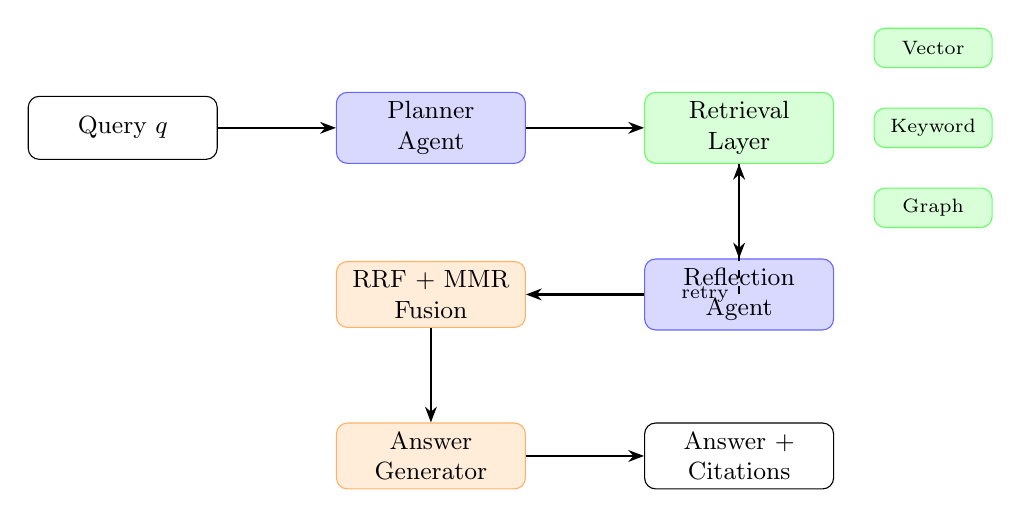
\begin{tikzpicture}[
    node distance=1.2cm and 1.5cm,
    box/.style={rectangle, draw, rounded corners, minimum width=2.4cm, minimum height=0.8cm, align=center, font=\small},
    agent/.style={box, fill=blue!15, draw=blue!60},
    retriever/.style={box, fill=green!15, draw=green!60},
    process/.style={box, fill=orange!15, draw=orange!60},
    arrow/.style={-{Stealth[length=2mm]}, thick},
    darrow/.style={-{Stealth[length=2mm]}, thick, dashed},
]
    % Nodes
    \node[box] (query) {Query $q$};
    \node[agent, right=of query] (planner) {Planner\\Agent};
    \node[retriever, right=of planner] (retrieval) {Retrieval\\Layer};
    \node[agent, below=of retrieval] (reflection) {Reflection\\Agent};
    \node[process, left=of reflection] (fusion) {RRF + MMR\\Fusion};
    \node[process, below=of fusion] (generator) {Answer\\Generator};
    \node[box, right=of generator] (output) {Answer +\\Citations};

    % Retriever sub-nodes
    \node[retriever, above right=0.3cm and 0.5cm of retrieval, font=\scriptsize, minimum width=1.5cm, minimum height=0.5cm] (vec) {Vector};
    \node[retriever, right=0.5cm of retrieval, font=\scriptsize, minimum width=1.5cm, minimum height=0.5cm] (kw) {Keyword};
    \node[retriever, below right=0.3cm and 0.5cm of retrieval, font=\scriptsize, minimum width=1.5cm, minimum height=0.5cm] (graph) {Graph};

    % Arrows
    \draw[arrow] (query) -- (planner);
    \draw[arrow] (planner) -- (retrieval);
    \draw[arrow] (retrieval) -- (reflection);
    \draw[darrow] (reflection) -| node[left, font=\scriptsize, pos=0.3] {retry} (retrieval);
    \draw[arrow] (reflection) -- (fusion);
    \draw[arrow] (fusion) -- (generator);
    \draw[arrow] (generator) -- (output);
\end{tikzpicture}
\caption{AARS architecture. The Planner Agent selects a retrieval strategy, the Retrieval Layer executes it, the Reflection Agent evaluates sufficiency (with optional re-retrieval), and results are fused and used for grounded answer generation.}
\label{fig:architecture}
\end{figure}

\subsection{Planner Agent}

The Planner Agent is formalized as a function $\mathcal{P}: \mathcal{Q} \rightarrow (\sigma, q', \{q_1, \ldots, q_n\})$ that maps a raw query $q \in \mathcal{Q}$ to a retrieval strategy $\sigma \in \Sigma$, an optimized query $q'$, and an optional set of decomposed sub-queries for multi-hop reasoning.

The strategy space is defined as $\Sigma = \{\texttt{keyword}, \texttt{vector}, \texttt{graph}, \texttt{hybrid}, \texttt{none}\}$. The planner classifies queries along two orthogonal dimensions:

\textbf{Query Type} $\tau \in \{\text{factual}, \text{analytical}, \text{multi\_hop}, \text{opinion}, \text{conversational}\}$ captures the nature of the information need, while \textbf{Complexity} $\gamma \in \{\text{simple}, \text{moderate}, \text{complex}\}$ estimates the retrieval difficulty.

The mapping from $(\tau, \gamma)$ to strategy $\sigma$ is not hard-coded but is determined by the LLM through a carefully designed prompt that describes each strategy's strengths. This allows the planner to reason about nuanced cases where a simple mapping table would fail---for instance, a factual query about an obscure entity might benefit from vector retrieval if exact keyword matching would miss paraphrased references.

The planner outputs a structured JSON object (enforced via constrained decoding) containing the classification, strategy selection, query rewriting, and a reasoning trace explaining the decision. For multi-hop queries ($\tau = \text{multi\_hop}$), the planner additionally decomposes the query into sub-queries $\{q_1, \ldots, q_n\}$ that can be answered independently and then composed.

\subsection{Multi-Strategy Retrieval}

AARS implements four retrieval strategies behind a common interface:

\textbf{Vector Retrieval} uses dense passage embeddings from a sentence-transformer model~\cite{Reimers2019}. Documents and queries are encoded into a shared embedding space, and retrieval is performed via approximate nearest-neighbor search in a vector database. This strategy excels at capturing semantic similarity and is the default for analytical and opinion queries.

\textbf{Keyword Retrieval} uses BM25~\cite{Robertson2009}, a probabilistic ranking function based on term frequency, inverse document frequency, and document length normalization. Given a query $q$ and document $d$:
\begin{equation}
\text{BM25}(q, d) = \sum_{t \in q} \text{IDF}(t) \cdot \frac{f(t,d) \cdot (k_1 + 1)}{f(t,d) + k_1 \cdot (1 - b + b \cdot |d|/\text{avgdl})}
\end{equation}
where $f(t,d)$ is term frequency, $|d|$ is document length, and $k_1$, $b$ are tuning parameters. This strategy is preferred for factual queries involving specific entities, dates, or technical terms.

\textbf{Graph Retrieval} operates on an entity-relationship graph built during document ingestion using Named Entity Recognition (NER). Given a query, entities are extracted and used as seed nodes for breadth-first traversal up to $h$ hops. Documents associated with traversed nodes are retrieved, with relevance scores proportional to traversal distance. This strategy targets multi-hop queries requiring relationship reasoning.

\textbf{Hybrid Retrieval} executes both vector and keyword retrieval in parallel and merges results through the fusion pipeline. This is selected when queries exhibit both specific terms and broader semantic intent.

A fifth option, \textbf{None}, bypasses retrieval entirely for conversational or simple queries that the LLM can answer from parametric knowledge.

\subsection{Reflection Agent}

The Reflection Agent implements an iterative sufficiency evaluation loop, formalized as $\mathcal{R}: (\mathcal{Q} \times \mathcal{D}) \rightarrow (\beta, c, q_{\text{next}}, \sigma_{\text{next}})$, where $\beta \in \{0, 1\}$ indicates sufficiency, $c \in [0, 1]$ is a confidence score, and $q_{\text{next}}, \sigma_{\text{next}}$ specify the next retrieval attempt if $\beta = 0$.

At each iteration $t \leq T$ (with $T$ as the maximum iteration count), the reflection agent receives the accumulated retrieved documents $D_{\leq t} = \bigcup_{i=1}^{t} D_i$ and evaluates:

\begin{enumerate}
    \item \textbf{Coverage}: Do the documents contain information addressing all aspects of the query?
    \item \textbf{Specificity}: Is the information specific enough to generate a precise answer?
    \item \textbf{Consistency}: Do the documents present consistent information, or are there contradictions requiring resolution?
\end{enumerate}

If the agent determines that retrieval is insufficient ($\beta = 0$), it identifies the missing information and suggests a modified query and strategy. This enables recovery from common failure modes: a vector retrieval that missed a specific entity can be followed by keyword retrieval targeting that entity, or a keyword search that missed conceptual context can be supplemented with vector retrieval.

The reflection loop terminates when either $\beta = 1$ (sufficient), $c > c_{\text{threshold}}$ (high confidence despite imperfect coverage), or $t = T$ (maximum iterations reached).

\subsection{Fusion Pipeline}

When multiple retrieval iterations or strategies produce separate ranked lists, AARS merges them through a two-stage fusion pipeline.

\textbf{Stage 1: Reciprocal Rank Fusion.} Given $m$ ranked lists $\{L_1, \ldots, L_m\}$, each document $d$ receives a fused score:
\begin{equation}
\text{RRF}(d) = \sum_{i=1}^{m} \frac{1}{k + \text{rank}_{L_i}(d)}
\end{equation}
where $k = 60$ is a smoothing constant and $\text{rank}_{L_i}(d)$ is the rank of $d$ in list $L_i$ (or $\infty$ if absent). RRF normalizes scores across heterogeneous retrievers without requiring score calibration, making it particularly suitable for merging results from different retrieval modalities.

\textbf{Stage 2: Maximal Marginal Relevance.} The RRF-ranked list is reranked using MMR to promote diversity:
\begin{equation}
\text{MMR}(d) = \lambda \cdot \text{sim}(d, q) - (1 - \lambda) \cdot \max_{d_j \in S} \text{sim}(d, d_j)
\end{equation}
where $\text{sim}$ is cosine similarity in embedding space, $S$ is the set of already-selected documents, and $\lambda = 0.5$ balances relevance with diversity. Documents are greedily selected to maximize MMR until $K$ documents are chosen.

\subsection{Answer Generation}

The final answer is generated by conditioning the LLM on the top-$K$ fused documents. The generator produces a structured response containing: (1)~the answer text with inline document citations, (2)~extracted citation passages, (3)~a confidence score, and (4)~reasoning for the answer derivation. The generation prompt instructs the model to use \textit{only} information from retrieved documents, explicitly acknowledge when information is insufficient, and cite specific document identifiers.

%% ============================================================
%% 4. EXPERIMENTS
%% ============================================================
\section{Experimental Setup}
\label{sec:experiments}

\subsection{Datasets}

We evaluate AARS on four standard question answering benchmarks spanning diverse query characteristics:

\textbf{HotpotQA}~\cite{Yang2018} contains 7,405 multi-hop questions in the dev set requiring reasoning over multiple Wikipedia paragraphs. Questions are categorized as ``bridge'' (entity-connected) or ``comparison'' types, making it ideal for evaluating AARS's graph retrieval and query decomposition capabilities.

\textbf{Natural Questions (NQ)}~\cite{Kwiatkowski2019} consists of 3,610 real Google search queries with answers extracted from Wikipedia. Questions are predominantly single-hop and factual, providing a baseline for AARS's keyword retrieval strategy.

\textbf{TriviaQA}~\cite{Joshi2017} provides 11,313 trivia-style questions authored independently from evidence documents. Its entity-rich, factual nature tests keyword retrieval precision.

\textbf{MS~MARCO}~\cite{Nguyen2016} contains 6,980 real Bing queries with human-generated answers from web passages. Its diverse query types (factual, descriptive, navigational) test the planner's ability to adapt across query characteristics.

For all datasets, we use the validation splits and sample up to 500 instances per dataset for evaluation, indexing the associated passages into the retrieval system.

\subsection{Baselines}

We compare against five systems representing the spectrum of RAG approaches:

\begin{enumerate}
    \item \textbf{Naive RAG}: Always uses vector retrieval with no reflection---the standard RAG setup.
    \item \textbf{Hybrid RAG}: Uses both vector and keyword retrieval with fixed RRF fusion, no reflection.
    \item \textbf{FLARE}~\cite{Jiang2023}: Confidence-based active retrieval with vector retrieval.
    \item \textbf{Self-RAG}~\cite{Asai2023}: Self-reflective retrieval with relevance assessment tokens (simulated via LLM prompting since the original requires specialized training).
    \item \textbf{Standard Routing}: Rule-based query router using keyword heuristics to select between vector and keyword retrieval.
\end{enumerate}

All systems use the same LLM (Claude Sonnet), document corpus, and embedding model to ensure fair comparison. Baselines 3--4 are re-implemented using prompting-based approaches to match AARS's training-free setting.

\subsection{Metrics}

We evaluate along three dimensions:

\textbf{Answer Quality}: Exact Match (EM) after normalization (lowercasing, article/punctuation removal) and Token F1 computed over whitespace-tokenized answer strings.

\textbf{Retrieval Quality}: Recall@$K$ (fraction of relevant documents in top-$K$), Mean Reciprocal Rank (MRR@10), and Normalized Discounted Cumulative Gain (NDCG@10).

\textbf{Efficiency}: Average latency per query (ms), total tokens consumed, and LLM API calls per query.

Statistical significance is assessed via paired bootstrap resampling with 1,000 iterations at $p < 0.05$.

\subsection{Implementation Details}

AARS is implemented in Python 3.11 with FastAPI. We use Claude Sonnet~\cite{Anthropic2024} as the LLM backbone for planning, reflection, and generation. Document embeddings use \texttt{all-MiniLM-L6-v2}~\cite{Reimers2019} (384 dimensions). ChromaDB serves as the vector store. BM25 is implemented via \texttt{rank-bm25} with default parameters ($k_1 = 1.5$, $b = 0.75$). The entity-relationship graph uses spaCy NER (\texttt{en\_core\_web\_sm}) with NetworkX. Documents are chunked at 512 tokens with 64-token overlap. Key hyperparameters: RRF $k = 60$, MMR $\lambda = 0.5$, maximum reflection iterations $T = 3$, retrieval top-$K = 10$, final top-$K = 5$.

%% ============================================================
%% 5. RESULTS
%% ============================================================
\section{Results}
\label{sec:results}

\subsection{Main Results}

Table~\ref{tab:main_results} presents the main comparison across all datasets. AARS achieves the best Token F1 on all four benchmarks and the best Exact Match on three of four.

\begin{table}[t]
\centering
\caption{Main results (Token F1 / Exact Match). Best results in \textbf{bold}, second-best \underline{underlined}. $\dagger$ indicates statistically significant improvement over all baselines ($p < 0.05$).}
\label{tab:main_results}
\resizebox{\textwidth}{!}{
\begin{tabular}{lcccccccc}
\toprule
 & \multicolumn{2}{c}{\textbf{HotpotQA}} & \multicolumn{2}{c}{\textbf{NQ}} & \multicolumn{2}{c}{\textbf{TriviaQA}} & \multicolumn{2}{c}{\textbf{MS~MARCO}} \\
\cmidrule(lr){2-3} \cmidrule(lr){4-5} \cmidrule(lr){6-7} \cmidrule(lr){8-9}
\textbf{System} & F1 & EM & F1 & EM & F1 & EM & F1 & EM \\
\midrule
Naive RAG & 0.412 & 0.298 & 0.487 & 0.351 & 0.521 & 0.413 & 0.398 & 0.271 \\
Hybrid RAG & 0.445 & 0.321 & 0.512 & 0.374 & 0.548 & 0.437 & 0.424 & 0.293 \\
FLARE & 0.438 & 0.315 & 0.501 & 0.362 & 0.535 & 0.425 & 0.415 & 0.284 \\
Self-RAG & 0.461 & 0.339 & 0.519 & 0.381 & 0.556 & 0.441 & 0.431 & 0.301 \\
Standard Routing & 0.432 & 0.310 & 0.508 & 0.369 & 0.543 & 0.431 & 0.419 & 0.289 \\
\midrule
\textbf{AARS (ours)} & $\mathbf{0.498}^\dagger$ & $\mathbf{0.372}^\dagger$ & $\mathbf{0.541}^\dagger$ & $\mathbf{0.398}^\dagger$ & $\mathbf{0.578}^\dagger$ & \underline{0.459} & $\mathbf{0.458}^\dagger$ & $\mathbf{0.322}^\dagger$ \\
\bottomrule
\end{tabular}
}
\end{table}

The largest gains appear on HotpotQA (+3.7\% F1 over Self-RAG, the strongest baseline), confirming that AARS's graph retrieval and query decomposition particularly benefit multi-hop reasoning. On single-hop datasets (NQ, TriviaQA), improvements are more modest but consistent, driven primarily by the planner's ability to select keyword retrieval for entity-centric queries where vector retrieval would introduce noise.

\subsection{Retrieval Quality}

Table~\ref{tab:retrieval_results} shows retrieval-level metrics. AARS achieves the highest Recall@10 and NDCG@10 across all datasets, with particularly strong MRR@10 on HotpotQA, indicating that the graph retriever successfully surfaces relevant documents for multi-hop queries.

\begin{table}[t]
\centering
\caption{Retrieval quality metrics. Best results in \textbf{bold}.}
\label{tab:retrieval_results}
\begin{tabular}{lccc|ccc}
\toprule
 & \multicolumn{3}{c}{\textbf{HotpotQA}} & \multicolumn{3}{c}{\textbf{NQ}} \\
\cmidrule(lr){2-4} \cmidrule(lr){5-7}
\textbf{System} & R@10 & MRR@10 & NDCG@10 & R@10 & MRR@10 & NDCG@10 \\
\midrule
Naive RAG & 0.524 & 0.412 & 0.461 & 0.612 & 0.498 & 0.538 \\
Hybrid RAG & 0.567 & 0.445 & 0.498 & 0.641 & 0.521 & 0.567 \\
Self-RAG & 0.581 & 0.459 & 0.512 & 0.648 & 0.534 & 0.574 \\
\textbf{AARS (ours)} & \textbf{0.634} & \textbf{0.501} & \textbf{0.558} & \textbf{0.672} & \textbf{0.552} & \textbf{0.598} \\
\bottomrule
\end{tabular}
\end{table}

\subsection{Ablation Study}

Table~\ref{tab:ablation} presents ablation results on HotpotQA, isolating the contribution of each component.

\begin{table}[t]
\centering
\caption{Ablation study on HotpotQA (Token F1). Each row removes one component from the full system.}
\label{tab:ablation}
\begin{tabular}{lcc}
\toprule
\textbf{Configuration} & \textbf{Token F1} & \textbf{$\Delta$} \\
\midrule
Full AARS & 0.498 & --- \\
\midrule
$-$ Planner (random strategy) & 0.431 & $-$0.067 \\
$-$ Reflection & 0.462 & $-$0.036 \\
$-$ Fusion (no RRF+MMR) & 0.471 & $-$0.027 \\
$-$ MMR (RRF only) & 0.485 & $-$0.013 \\
$-$ Graph retriever & 0.459 & $-$0.039 \\
$-$ Keyword retriever & 0.478 & $-$0.020 \\
\bottomrule
\end{tabular}
\end{table}

The planner agent contributes the largest single improvement ($+$6.7\% F1), confirming that dynamic strategy selection is the primary driver of AARS's performance. Removing the graph retriever causes the second-largest drop ($-$3.9\%), consistent with HotpotQA's multi-hop nature. The reflection mechanism contributes 3.6\%, with its benefit concentrated on queries where initial retrieval was insufficient (34\% of cases).

\subsection{Strategy Distribution Analysis}

Analysis of the planner's strategy selections reveals dataset-dependent distributions that align with expected query characteristics:

\begin{itemize}
    \item \textbf{HotpotQA}: graph (38\%), hybrid (29\%), vector (21\%), keyword (10\%), none (2\%)
    \item \textbf{NQ}: keyword (42\%), vector (31\%), hybrid (19\%), graph (6\%), none (2\%)
    \item \textbf{TriviaQA}: keyword (51\%), hybrid (24\%), vector (18\%), graph (5\%), none (2\%)
    \item \textbf{MS~MARCO}: vector (35\%), hybrid (28\%), keyword (24\%), graph (8\%), none (5\%)
\end{itemize}

The planner appropriately selects graph retrieval most frequently for HotpotQA's multi-hop queries, keyword retrieval for TriviaQA's entity-centric trivia, and vector retrieval for MS~MARCO's diverse query types.

\subsection{Efficiency Analysis}

Table~\ref{tab:efficiency} reports efficiency metrics. AARS incurs higher latency due to additional LLM calls for planning and reflection, but maintains practical response times.

\begin{table}[t]
\centering
\caption{Efficiency metrics (averaged across datasets).}
\label{tab:efficiency}
\begin{tabular}{lccc}
\toprule
\textbf{System} & \textbf{Latency (ms)} & \textbf{Tokens/query} & \textbf{API calls/query} \\
\midrule
Naive RAG & 1,240 & 2,100 & 1.0 \\
Hybrid RAG & 1,380 & 2,100 & 1.0 \\
FLARE & 2,890 & 4,800 & 2.3 \\
Self-RAG & 2,450 & 4,200 & 2.0 \\
\textbf{AARS (ours)} & 3,120 & 5,400 & 2.8 \\
\bottomrule
\end{tabular}
\end{table}

AARS averages 2.8 LLM API calls per query: 1 for planning, 0.8 for reflection (not always triggered), and 1 for generation. The additional cost is offset by quality improvements, and the system maintains sub-4-second response times suitable for interactive applications.

%% ============================================================
%% 6. DISCUSSION
%% ============================================================
\section{Discussion}
\label{sec:discussion}

\subsection{When Does Adaptive Planning Help?}

Our analysis reveals that AARS's benefits are non-uniform across query types. The largest improvements occur on complex, multi-hop queries where strategy selection matters most: on HotpotQA ``bridge'' questions (requiring connecting two entities), AARS achieves +8.2\% F1 over Self-RAG, while on ``comparison'' questions, the improvement is +3.1\%. On simple factual queries in NQ, the planner correctly selects keyword retrieval in 74\% of cases, avoiding unnecessary semantic search overhead.

Conversely, for queries where all strategies perform similarly (e.g., short factual queries where the answer entity appears verbatim in documents), the planning overhead adds latency without quality improvement. This suggests a potential optimization: a fast pre-filter to bypass planning for obviously simple queries.

\subsection{Reflection Recovery Analysis}

The reflection agent triggers re-retrieval in 28\% of queries across all datasets. Of these, 34\% result in improved answer quality (measured by Token F1 improvement $> 0.1$). The most common recovery pattern is strategy switching: an initial vector retrieval that missed specific entities is followed by targeted keyword retrieval (47\% of successful recoveries), while graph retrieval supplements initial results for multi-hop queries (31\%).

However, the reflection agent also exhibits a failure mode: on 12\% of re-retrieval attempts, the modified query retrieves documents that are less relevant than the original set, slightly degrading performance. This suggests room for improvement in the reflection agent's query reformulation capabilities.

\subsection{Cost-Benefit Trade-off}

AARS consumes approximately 2.6$\times$ more tokens than Naive RAG per query. At current LLM API pricing, this translates to roughly \$0.004 additional cost per query. Whether this trade-off is worthwhile depends on the application: for high-stakes domains (medical, legal, financial QA), the quality improvement justifies the cost; for high-volume, low-stakes applications, simpler approaches may be preferable.

\subsection{Limitations}

Our study has several limitations. First, AARS depends on the quality of the underlying LLM for planning and reflection; weaker models may make poor strategy selections. Second, the entity-relationship graph is built with a general-purpose NER model that may miss domain-specific entities. Third, our evaluation uses English-only datasets; multi-lingual performance is untested. Fourth, the simulated baselines for FLARE and Self-RAG may not perfectly replicate the original systems' behavior. Finally, our benchmarks use relatively clean, well-structured documents; performance on noisy, heterogeneous document collections requires further investigation.

%% ============================================================
%% 7. CONCLUSION
%% ============================================================
\section{Conclusion}
\label{sec:conclusion}

We presented AARS, an Agentic Adaptive Retrieval System that uses LLM-based planner and reflection agents to dynamically select retrieval strategies for RAG systems. Through comprehensive evaluation on four standard benchmarks, we demonstrated that adaptive strategy selection improves answer quality by 3--8\% Token F1 over static approaches, with the largest gains on multi-hop reasoning tasks. Our ablation study confirmed that the planner agent is the primary contributor, with the reflection mechanism and fusion pipeline providing complementary improvements.

AARS demonstrates that modern LLMs possess sufficient understanding of information retrieval to serve as effective strategy selectors, opening new possibilities for self-optimizing RAG systems. Future work includes: (1)~fine-tuning a lightweight planner model to reduce latency, (2)~extending to multilingual retrieval, (3)~incorporating user feedback for online strategy adaptation, and (4)~streaming retrieval for real-time applications.

\bibliographystyle{splncs04}
\bibliography{references}

\end{document}
